% -*- root: ../main.tex -*-
\chapter{Design Architetturale}
Dopo un'attenta analisi dei requisiti, si è proceduto con la fase di \textbf{design architetturale} che si è sviluppata in più passi, partendo dalla definizione ad alto livello di un'architettura generale e \textbf{raffinandola} gradualmente. 

	
\section{Architettura Generale}
Il primo passo per quanto riguarda l'aspetto della \textbf{progettazione} è consistito nella ricerca dei pattern più adatti da applicare, nell'individuazione dei principali componenti dell'\textbf{architettura generale}, e nella definizione dei modi in cui essi interagiscono.

La seguente immagine (fig: \ref{fig:architectureClassDiagram}) definisce il \textbf{core} dell'architettura generale che è stato successivamente \textbf{ampliato} per gestire anche la parte di architettura \textbf{client-server} necessaria alla realizzazione della modalità \textbf{multiplayer}.
\begin{figure}[H]
	\centering
	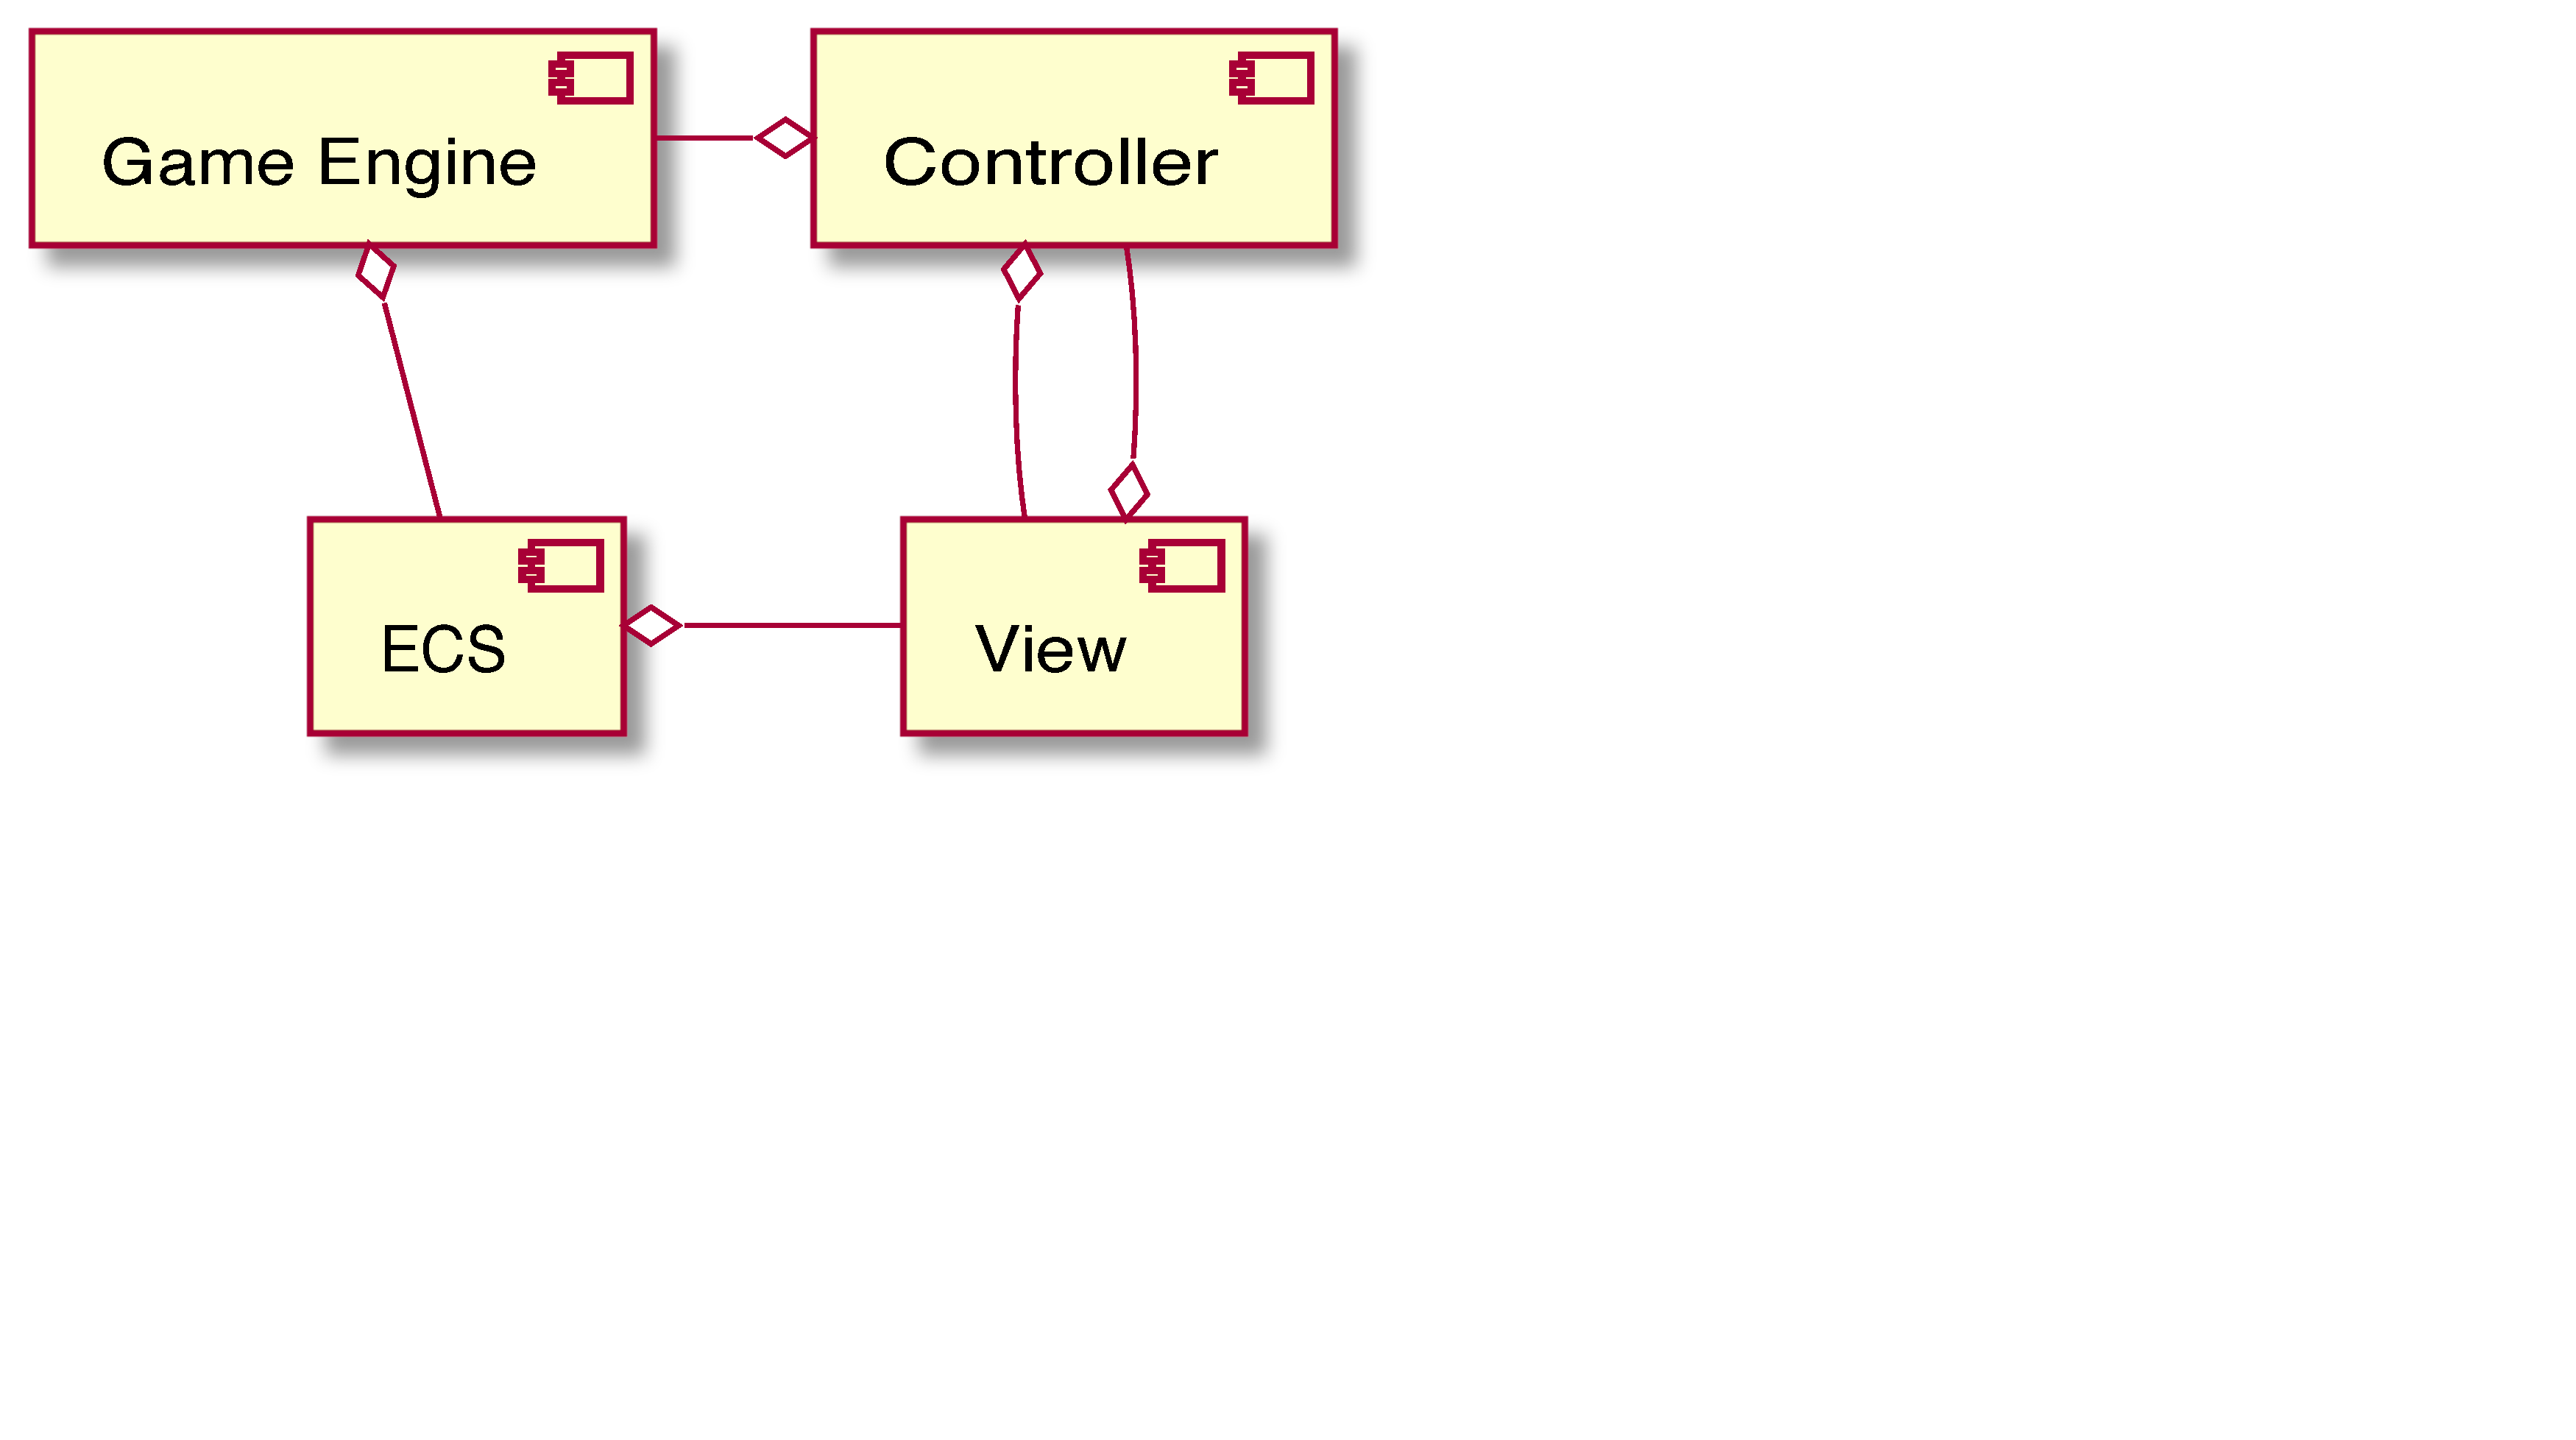
\includegraphics[width=0.80\columnwidth]{plantuml/rendered/classDiagrams/architectureClassDiagram.pdf}
	\caption{Diagramma raffigurante le entità principali dell’architettura e le loro interazioni ad un alto livello di astrazione.}
	\label{fig:architectureClassDiagram}
\end{figure}

Spiegazione breve delle entità in gioco

\begin{itemize}
    \item \textbf{View:} ha l'obbiettivo di fornire all'utente una \textbf{schermata} intuitiva per il controllo del gioco.
    \item \textbf{Controller:} rappresenta il punto di \textbf{snodo} per la gestione della logica principale dell'applicazione. La sua funzione primaria è quella di gestire la \textbf{comunicazione} tra: View, ECS, e GameEngine.
    \item \textbf{ECS:} è un aggregato di \textbf{sistemi}, \textbf{entità} e \textbf{componenti} che esprimono e contengono in maniera astratta la logica di gioco.
    \item \textbf{GameEngine:} rappresenta il cuore del gioco; incapsula il flusso di controllo principale e tramite ECS calcola continuamente il nuovo ambiente.
\end{itemize}

\section{Pattern Architetturali Utilizzati}
\subsection{ECS}
Trattandosi dello sviluppo di un videogioco, per il quale è necessario creare un motore di gioco, è stato scelto di utilizzare il pattern architetturale \textbf{Entity-Component-System} (ECS). Questo pattern è largamente utilizzato nello svi-luppo di videogiochi per motivi di performance e per la sua estensibilità e manutenibilità.

ECS si compone di tre parti principali:
\begin{itemize}
    \item \textbf{Entità:} rappresentano gli elementi in gioco, ad esempio Bumper car, PowerUp o Enemy. Ad ogni entità vengono associati uno o più componenti.
    \item \textbf{Componenti:} sono delle proprietà che vengono possedute da una o più entità e ne rappresentano lo stato. Esempi di possibili componenti sono direzione o posizione. 
    \item \textbf{Sistemi:} definiscono dei comportamenti necessari a gestire dei sottoinsiemi della logica di gioco. Gestiscono le interazioni tra le entità agendo sui componenti associati ad esse.
\end{itemize}


\subsection{MVC}
Il pattern \textbf{MVC} rappresenta uno standard per quanto riguarda il \textbf{design} di applicazioni \textit{robuste} ed \textit{estendibili}. Nel nostro caso il pattern è stato utilizzato in concomitanza con il pattern \textbf{ECS} permettendo così di raggiungere una maggiore \textbf{separazione dei concetti}. L'MVC progettato si compone dei seguenti moduli:
\begin{itemize}
    \item \textbf{Model:}
    All'interno del nostro applicativo esistono due tipi di modello:
    \begin{itemize}
        \item \textbf{Game Model:}
        Il \textbf{modello di gioco} rappresenta l'insieme delle \textbf{strutture dati} utili per modellare il gameplay. Nel nostro caso questo compito è stato catturato interamente dal \textbf{pattern ECS}.
        \item \textbf{Application Logic Model:}
        Il modello della  \textbf{logica applicativa} riguarda tutti i dati utili al \textbf{corretto funzionamento} dell'applica-zione (Impostazioni, Livelli, Dati utente, ecc).
    \end{itemize}
    \item \textbf{View:}
    L'interfaccia grafica si configura  come un \textbf{punto di intersezione} fra \textbf{ECS} e \textbf{MVC} per quanto riguarda gli aspetti dell'interazione utente. Essa si compone di due tipologie di schermate:
    \begin{itemize}
        \item \textbf{Game Screen:}
        È una schermata di gioco connessa interamente al modulo ECS. Essa ha come scopo principale quello di mostrare gli \textbf{aggiornamenti di gioco} e acquisire i \textbf{comandi} da parte dell'utente.
        \item \textbf{Application Screen:}
        È istanza di una semplice \textbf{schermata di presentazione}. Lo scopo di una application screen consiste essenzialmente nel garantire all'utente una buona \textbf{usabilità} e \textbf{interazione} col sistema, incapsulando le informazioni di modello in una \textbf{visualizzazione fruibile}. 
    \end{itemize}
    \item \textbf{Controller:}
    Gestisce le \textbf{interazioni} fra i principali moduli dell'architet-tura e mette a disposizione una serie di \textbf{funzionalità} relative alla \textbf{gestione delle risorse}.
\end{itemize}

\subsection{Client-Server} 
Un'architettura di tipo client-server si è resa necessaria per poter gestire la modalità di gioco \textbf{multiplayer}. Il sistema deve infatti permettere ad un utente di \textbf{ospitare} una partita assumendo il ruolo di \texttt{server} e ad altri utenti di \textbf{partecipare} ricoprendo il ruolo di \texttt{client}. 

\subsubsection{Scelta del paradigma}
Per gestire l'interazione tra Client e Server si è ritenuto adatto l'utilizzo del \textbf{paradigma ad attori} applicato mediante la modellazione di un attore \texttt{Server} e un attore \texttt{Client} che interagiscono tramite scambio di \textbf{messaggi}. 

\subsubsection{Distribuito vs centralizzato}
Quando ci si cimenta nella progettazione di un sistema che si interfaccerà in \textbf{rete} è necessario definire quale \textbf{approccio} utilizzare. Essenzialmente vi sono due strade percorribili: una basata su uno schema \textbf{centralizzato} mentre l'altra basata su uno schema \textbf{peer-to-peer}.
\begin{itemize}
    \item Approccio centralizzato
        \begin{itemize}
        \setlength\itemsep{0em}
        \item Semplicità
        \item Reattività
        \item Consistenza
        \item Single Point of Failure
    \end{itemize}
    
    \item Approccio distribuito
        \begin{itemize}
        \setlength\itemsep{0em}
        \item Fault-tolerance
        \item Carico suddiviso
        \item Modulare
        \item Complesso
        \item Incline all'inconsistenza
        
    \end{itemize}
\end{itemize}
Si è preferito utilizzare un approccio centralizzato anziché distribuito perché, data la natura del sistema che è da realizzare, si è ritenuto che una scelta diversa avrebbe portato, a fronte di un maggiore sforzo progettuale e implementativo, a dei risultati peggiori in termini di performance, reattività e consistenza.


Come mostrato dalla figura \ref{fig:clientServerComponentDiagram} il sistema è stato progettato in modo da poter estendere l'architettura core per il multiplayer, "staccando" l'engine del client e sostituendolo con l'attore client che poi comunicherà con l'attore server, che si interfaccia direttamente con il server.
\begin{figure}[H]
	\centering
	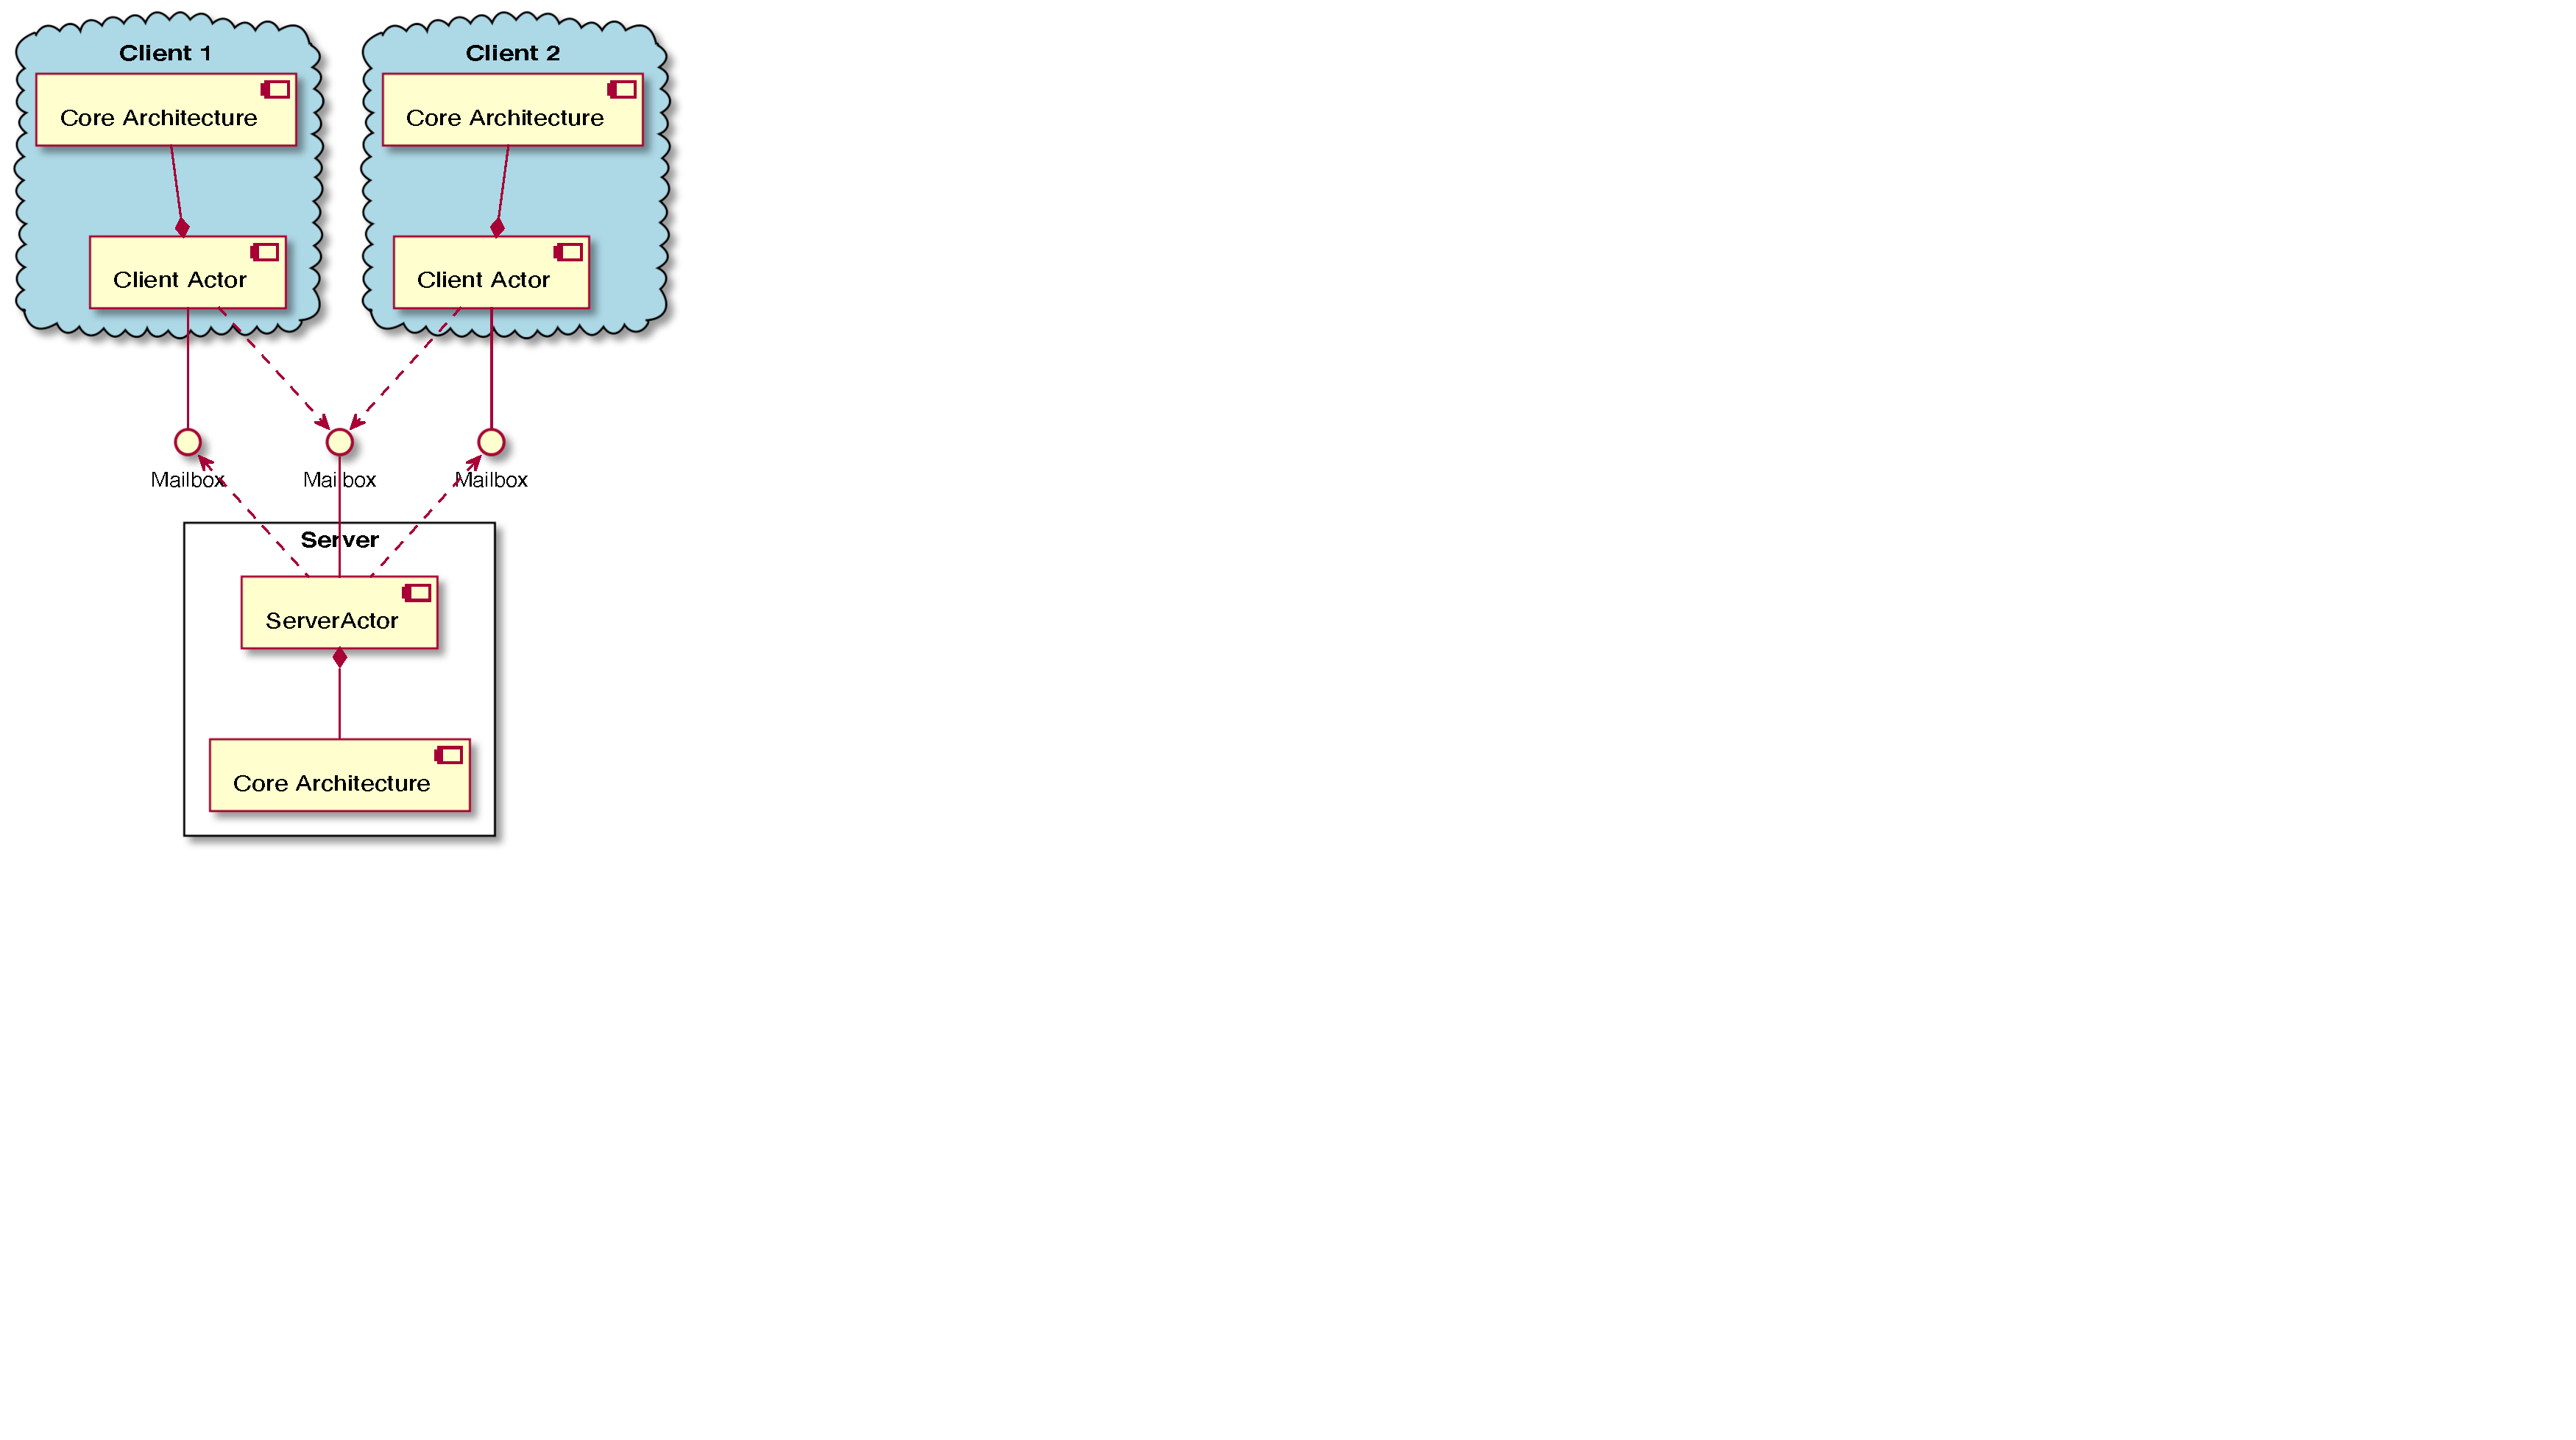
\includegraphics[width=0.70\columnwidth]{plantuml/rendered/componentDiagrams/clientServerComponentDiagram.pdf}
	\caption{Diagramma raffigurante gli attori di tipo Client e Server e le loro interazioni.}
	\label{fig:clientServerComponentDiagram}
\end{figure}

\section{Scelte Tecnologiche Cruciali}
    \subsection{Akka} 
        Per l'implementazione del paradigma ad attori sì e scelto di utilizzare \textbf{Akka} come layer di \textbf{comunicazione} nello sviluppo del multiplayer. Akka garantisce un'ottima \textbf{scalabilità} e un buon livello di \textbf{astrazione}, che permette di gestire la comunicazione in maniera più trasparente rispetto ai classici metodi basati sulle \textbf{socket}. Il modello \textbf{Client-Server} basato su Akka risulta così di facile \textbf{implementazione}.
        
        Inoltre, il fatto che Akka sia implementato in \textbf{Scala} rende più semplice e naturale l'utilizzo del framework. 